\chapter{The \telemacsystem{} development plan}
\label{devplan}

The development plan describes explicitly all the processes on the software
during the life cycle of the \telemacsystem{} code and ensures its Quality.\\

The \telemacsystem{} activity is decomposed into three main activities that are
described in Chapter~\ref{devact}:
\begin{itemize}
\item \textbf{Development activity}.
\item \textbf{Verification and Validation activity}.
\item \textbf{Release activity}.
\end{itemize}

\section{Rights to commit new developments}

People involved in the development of the \telemacsystem{} can be divided into
the following groups:
\begin{itemize}
\item \textbf{The \telemacsystem{} development team (TDT)}: to be a part of the
  TDT you need to have writing access on the GitLab repository. To be in
  the development team, the developer must have read the developer guide and
  the SQP in order to apply it to its future developments. The PM is a member
  of the TDT\@.
\item \textbf{Developers from EDF units}: they are developers from one of the
  group of EDF and are developing for the \telemacsystem{} project. It is
  recommended that they follow the \telemacsystem{} workshop. They will need to
  contact a member of the TDT to integrate their development.
\item \textbf{Non EDF developers working with EDF}: they can be subcontractors,
  interns, PhD students or any other partners working with EDF\@. It is also
  recommended that they follow the \telemacsystem{} workshop. The follow-up of
  the development will have to be done by a members of the TDT\@.
\item \textbf{Open source community, academic and industrial partners}:
  The \telemacsystem{} is an open source code under GNU-GPL\@. Anyone can get
  the source and develop their own version. But for a development to be
  integrated into the official version, it must be studied by the TDT and
  follow the process described in~\ref{dev}. If the integration is validated,
  the delivery of the evolution for the code must go through a member of the
  TDT\@ (See~\ref{devint}).
\end{itemize}

\section{Life cycle of a development}

\subsection{Definition of a development}
\label{defdev}

A development represents a modification on the source code of the
\telemacsystem{}, its documentation and its dedicated tools. (i.e.\ everything
that is under the configuration, see~\ref{conf}). The developments are
classified into three types of maintenance:
\begin{itemize}
\item \textbf{Evolution maintenance}: this maintenance aims to upgrade the
  software in order to:
  \begin{itemize}
  \item Break limits of some existing functionalities (performance, strength,
    precision\ldots).
  \item Develop new functionalities to satisfy new needs or demands.
  \end{itemize}
  These evolutions can be developments of new features made by one of EDF
  Units. They can also originate from an outside developer and been brought in
  by the PM\@.
  Each evolution must be associated with a GitLab issue and merge request.
  This allows the PM to get a general overview of the work in progress.
  Depending on the size of the development, it can even be presented by the
  developer in an ADEPHE meeting. This allows the TDT to evaluate the impact of
  the development and maybe advise the developer on what to do. The development
  must be validated by one of the CHs.
\item \textbf{Corrective maintenance}: the corrective maintenance is the
  removal of an anomaly in the code or documentation. Such an anomaly can be:
  \begin{itemize}
  \item A problem in the code, a mistake in the documentation, an error in the
    GUI\@.
  \item An error in a test case detected during the Verification and Validation
    process.
  \item A problem in the implementation detected by user.
  \end{itemize}
  Corrective maintenance must also be coupled with a GitLab issue and merge
  request if the fix is also to be applied to the current stable version.
\item \textbf{Adaptive maintenance}: the adaptive maintenance concerns
  evolution in the code in order to comply with a change of environment
  (Operating System, compiler, new cluster\ldots).
\end{itemize}

\subsection{Life cycle of a \telemacsystem{} development}
\label{lifecycle}
The life cycle of a \telemacsystem{} development follows a list of steps shown
on the Figure~\ref{cycle}. Those steps will be described in the next sections.

\begin{figure}[H]
\centering
\begin{tikzpicture}[node distance = 1cm, auto]
  % Defining style for the task
  \tikzstyle{task} = [draw, very thick, fill=white, rectangle]
  \tikzstyle{bigbox} = [draw, thin, rounded corners, rectangle]
  \tikzstyle{box} = [draw, thick, fill=white, rounded corners, rectangle]
  % Creation of the nodes
  \node (ISSUE) [task] {1. Issue on GitLab};
  \node (CHs) [task, below of=ISSUE] {2. CHs};
  \node (IMPL) [task, below of=CHs] {3. Implementation};
  \node (null2) [right of=IMPL, node distance=9em] {};
  \node (VV) [task, below of=IMPL] {4. Verification \& Validation};
  \node (DOC) [task, below of=VV] {5. Documentation};
  \node (INT) [task, below of=DOC] {6. Integration};
  \node (null1) [right of=INT, node distance=9em] {};
  \node (null3) [left of=INT, node distance=9em] {};
  \node (MAIN) [box, below of=INT, node distance=4em] {Main branch of \telemacsystem{}};
  % big box
  \node (DEV) [bigbox, fit = (ISSUE) (CHs) (IMPL) (null1) (null2) (null3) (VV) (DOC) (INT)] {};
  \node at (DEV.north) [above, inner sep=3mm] {\textbf{Development}};
  % Creation of the path between the nodes
  \draw[->] (ISSUE) to node {} (CHs);
  \draw[->] (CHs) to node {} (IMPL);
  \draw[->] (IMPL) to node {} (VV);
  \draw[->] (VV) to node {} (DOC);
  \draw[->] (DOC) to node {} (INT);
  \draw[-] (INT) -- node [near start] {no} (null1.center);
  \draw[-] (null1.center) -- (null2.center);
  \draw[->] (null2.center) -- node [near start] {} (IMPL);
  \draw[->] (INT) to node {yes} (MAIN);
\end{tikzpicture}
\caption{\label{cycle}Life cycle of a \telemacsystem{} development}
\end{figure}

Depending on the kind of development (corrective, adaptive, evolution
maintenance) some of those steps can be skipped.
The different steps are:
\begin{enumerate}
\item Proposal step.
\item Examination and impact study step.
\item Implementation step.
\item Verification step.
\item Documentation step.
\item Approbation and validation step.
\end{enumerate}

This development cycle is based on a V scheme life cycle, it contains those
different steps and the different types of testing (see next paragraph). To be
more precise, it is more of spiral cycle in which the V cycle is read
iteratively in order to improve the quality gradually.

\section{Description of the development steps}
\label{dev}

\subsection{Proposal step}

Every demand must go through the proposal step, may it be a corrective,
adaptive, evolution maintenance (see Section~\ref{defdev} for a definition).\\

This proposal is given to the TDT by creating a new GitLab issue
(\url{https://gitlab.pam-retd.fr/otm/telemac-mascaret/-/issues}).\\

The goal of this proposal is to:
\begin{itemize}
\item Inform the CHs of the proposed development.
\item Give more information on the impact in the software.
\item Plan and organise the resources for the development.
\item To prepare the validation in ADEPHE if necessary.
\end{itemize}

\textbf{In charge}: the proposer.

\textbf{Documents}: the GitLab issue.

\subsection{Job repartition step}

When the GitLab issue is published, the CHs have to determine if the
development must be followed by the TDT\@. This mainly concerns evolution
maintenance but can also concern corrective maintenance if it has a major
impact on the code.\\

The goal of this step is:
\begin{itemize}
\item If it is an evolution maintenance, to verify the coherence of the
  evolution with: the kernel, the existing, in development or planned
  functionalities, the functionality itself, the modifications needed in the
  data structure, the architecture of the code or the GUI, the name of the new
  keywords and structure. In particular guiding the developer towards a reusing
  of existing routines.
\item In case of a corrective maintenance it studies the impact on the
  Verification and Validation process.
\item To help the developer in its choice of algorithm and implementation.
\item To discuss the test cases for Verification and Validation.
\item To estimate the impact on the documentation.
\end{itemize}

\textbf{In charge}: CHs, TDT, handler of the development.

\textbf{Documents}:
\begin{itemize}
\item Input: the GitLab issue.
\item Output: update of evolution on the issue.
\end{itemize}

\subsection{Implementation step}

This is the coding part of what was specified in the GitLab issue, with the
modifications that the discussion during the ADEPHE could have generated.\\

The developer must follow the coding conventions given in the developer guide
of the \telemacsystem. All the developments are done under a version control
tool. For for each development, a branch dedicated to that development needs to
be created and a GitLab merge request 
(https://gitlab.pam-retd.fr/otm/telemac-mascaret/-/merge\_requests)
must be opened to keep track of the development updates.\\

The control of the implementation is made by running the \telemacsystem{}
validation. When possible, in the case of evolutionary maintenance, it is
preferable to add a test case that checks the new functionalitiy, if one does
not exist.\\

The development must be done on a branch and follow the development version (or
main, see section~\ref{conf} for a definition). It is strongly recommended to
keep up to date with the development version as often as possible. This lessens
the workload of that process compared to what would need to be done at the end
of the development.\\

It is also recommended to use developer tools during the development, such as a
debugger (GDB, TotalView), a memory leak detector (valgrind) and a code editor
(Atom, Emacs, Visual Studio Code\ldots) or an IDE (Code::Blocks, Visual
Studio\ldots)\\

The GitLab merge request is updated as the implementation goes on.\\

\textbf{In charge}: the developer.

\textbf{Documents}:
\begin{itemize}
\item Input: GitLab issue and merge request, developer manual, verification and
   validation test cases.
\item Output: source code, test cases, results of tests.
\end{itemize}

\subsection{Verification step}

The Verification and Validation process is deeply linked with the
implementation process. This process aims to verify the code at the level of
the algorithm and the whole model using the Verification and Validation test
cases (even if a small part of the code has been modified, like during a
corrective and adaptive maintenance). This is then complementary (even
redundant) with the verification done during the implementation. The
Verification and Validation process is explained in Chapter~\ref{vv}.\\

As mentioned in the previous paragraph, every development must contain
Verification and Validation test cases:
\begin{itemize}
\item Evolution maintenance: for an evolution of the code at least one
  Verification and one Validation case must be added if existing cases cannot
  be used. The choice of those cases are discussed with the TDT\@.
\item Corrective and adaptive maintenance: All the test cases must be rerun.
\end{itemize}

\textbf{In charge}: the developer.

\textbf{Documents}:
\begin{itemize}
\item Input: GitLab issue and merge request, validation manual.
\item Output: update of GitLab issue and merge request, \LaTeX\xspace the
  documentation follows the validation standard for each test case.
\end{itemize}

\subsection{Documentation step}

The \telemacsystem{} technical documentation is composed of the following manuals:
The five below are duplicated for each the \telemacsystem{} module.
\begin{itemize}
\item \textbf{Reference Manual}: describes every keyword in the dictionary of
  one module.
\item \textbf{Theory guide}: describes the physical phenomena modelled by the
  module and the numerical methods used to solve the equations modelling these
  phenomena.
\item \textbf{Validation Manual}: presents a list of test cases which validate
  the conceptual model, algorithms and software implementations. It is a
  concatenation of all the test case documentation for one module.
\item \textbf{User Manual}: describes how to use the code.
\end{itemize}

\begin{itemize}
\item \textbf{Online Manual (Doxygen)}: this documentation is linked with the
  source code (it is built by using special comment written in the source
  code). It describes the functions and structures of the source code.
\item \textbf{Developer Manual}: describes all the actions a developer might
  have to do during a development. It also defines the programming convention.
\item \textbf{NEWS.txt}: for every release, lists the new functionalities and
  corrections.
\end{itemize}

The documentations are under a configuration handler (Git) in \LaTeX\xspace
format. The documentation is under the responsibility of the Doc Handler and
the CHs.

Depending on the type of development, a few cases can occur:
\begin{itemize}
\item \textbf{Evolution Maintenance}: for a new functionality of the code, a
  new section must be added in the theory guide describing the new physics and
  in the user manual showing how to use that functionality. The Online
  documentation as well as the \textbf{NEWS.txt} file must also be updated.
\item \textbf{Corrective, adaptive Maintenance}: if the development has an
  impact on the documentation, it must be updated by the developer. If the
  development is to be merged on the version branch, the \textbf{NEWS.txt} file
  should also be updated.
\end{itemize}

In any case, the modification must go through the Doc Handler and must be
validated by the CHs and the PM\@.\\

\textbf{In charge}: the Doc Handler.

\textbf{Documents}:
\begin{itemize}
\item Input: all the documentation.
\item Output: the updated documentation.
\end{itemize}

\subsection{Integration step}

The integration step concerns the restitution of a development into the
main branch of the \telemacsystem{} (main, see~\ref{conf}).\\

The integration step is composed of the following steps:
\begin{itemize}
\item Designing the member of the TDT in charge of the integration of the
  development.
\item Integration of the Verification and Validation cases under the
  supervision of the V\&V Handler.
\end{itemize}

Not following those steps allows the CHs to refuse the integration and even
remove it from the development version.\\

\textbf{Presentation of the development in ADEPHE}

The ADEPHE meetings are monthly.
To be allowed in ADEPHE, a developer must have:
\begin{itemize}
\item Synchronized their branch with the latest version of the main branch.
\item Verified that the code follows the programming rules.
\item Added the new test cases for the development.
\item Validated their branch using the validation tools (CIS).
\item Updated the GitLab merge request.
\end{itemize}

During the ADEPHE, the person in charge of the development must present:
\begin{itemize}
\item The development and how it was implemented: the functionalities if it is
  an evolution maintenance, in case of a corrective, adaptive maintenance: the
  data structure, the new keywords, how to use it.
\item The Verification and Validation cases and their results.
\item The impact on the documentation.
\end{itemize}

At the end of the presentation the TDT must decide:
\begin{itemize}
\item The integration or the dismissal of the development in the main branch.
\item The integration or the dismissal of the test case.
\item The integration or the dismissal of the modifications on the
documentation.
\item The person in charge of the integration.
\end{itemize}

In case of a disagreement in the TDT the PM has the final word.

\textbf{In charge}: CHs, TDT\@.

\textbf{Documents}:
\begin{itemize}
\item Input: GitLab merge request, documentation.
\item Output: update of the GitLab merge request.
\end{itemize}

\textbf{Integration}

After the green light of the TDT, the person in charge of the integration has
to do the following actions:
\begin{itemize}
\item Accept the merge request.
\item Close the GitLab issue.
\end{itemize}

\textbf{In charge}: TDT\@.

\textbf{Documents}:
\begin{itemize}
\item Input: GitLab merge request.
\item Output: update of GitLab merge request, documentation, sources.
\end{itemize}

\subsection{Checklists for Developer and for Integrator}

To summarise the step that were explained before here is a checklist of the
actions he will have to do:
\begin{todolist}
\setlength\itemsep{0.01em}
\item Create a GitLab issue (on https://gitlab.pam-retd.fr/otm/telemac-mascaret/-/issues).
\item Discuss with TDT\@.
\item Update the main branch to the latest version.
\item Create a development branch to work on.
\item Do the work.
\item Update the documentation.
\item Update \verb!NEWS.txt! to reflect the changes.
\item Add test cases to test the development (with documentation, graphics and
  validation).
\item Run \verb!compile_telemac.py --check! (to check Fortran coding conventions).
\item Run \verb!pylint! (to check Python coding conventions).
\item Run \verb!compile_telemac.py --clean --rescan! and update cmdf files accordingly.
\item Run \verb!compile_telemac.py --clean! for normal and debug configuration.
\item Run \verb!validate_telemac.py! for normal and debug configuration.
\item Run \verb!validate_telemac.py --notebook! for normal and debug configuration.
\item Run \verb!doc_telemac.py! if there are any modifications in the documentation.
\item Run \verb!damocles.py --eficas! if there are any modifications in the
  dictionaries.
\item Submit a merge request and assign it to the integrator.
\end{todolist}


The following checklist describes the actions that the integrator must follow:
\begin{todolist}
\setlength\itemsep{0.01em}
\item Check that the GitLab issue and merge request are properly filled.
\item Check that the code follows the coding conventions.
\item Check that the test cases are appropriate.
\item Check that the implementation of the solution is good.
\item Check that the development is up to date with the main branch.
\item Check that the \verb!NEWS.txt! file has been updated.
\item Check that the branch has been cleaned of redundant commits using
  Git interactive rebase.
\item Accept the merge request.
\end{todolist}


\section{Maintenance}

In this part, the maintenance concerns only the corrective and adaptive
maintenance.\\

The \telemacsystem{} project is in charge of the non-regression of the
\telemacsystem{} functionalities on the Verification and Validation test
base.\\

The \telemacsystem{} project is also in charge of the adaptive maintenance (see
Section~\ref{defdev}).\\

The project in charge of other developments is in charge of the corrective
maintenance for their developments. But a help from the TDT is possible in
case of big difficulties. If the bug is easy to correct the TDT can, with the
authorisation of the person on charge, correct the bug themselves.\\

In any case the development must follow the development step described in
Section~\ref{lifecycle} and summarised in Figure~\ref{cycle}.\\

If the bug is also in the latest version branch, it should also be merged there
and an issue and merge request must be created.\\

\textbf{Removal of a functionality}

The CHs can decide to remove a functionality if it has become obsolete or
irrelevant. This decision must be validated by the PM\@. The CHs must warn the
user community.\\

The removal of a functionality can only happen on the main branch, it is not
retroactive.\\

The removal of a functionality concerns:
\begin{itemize}
\item The source code and the linked library.
\item If there are any, the impacted verification and validation.
\item The documentation.
\end{itemize}

\section{Integration of development from the open-source community}
\label{devint}

An integration from the open-source community must follow the same process as
an internal development.

\section{Configuration management}
\label{conf}

\subsection{Version control}

The different versions of the elements of the \telemacsystem{} software are
handled by a version control tool. Such a tool allows to track the evolutions
of the source code and ease the collaboration between multiple developers\@.\\

The version control tool that is used for the \telemacsystem{} is Git, which 
allows to clone any revision of the source code with the entire modification
history. The official Git repository of the software is hosted on a GitLab
server and is accessible at the following URL:
\url{https://gitlab.pam-retd.fr/otm/telemac-mascaret}.

\subsection{Elements under version control}

The elements of the \telemacsystem{} software concerned by the version control
are the source code, the environment scripts, the documentation and the test
cases.

\subsection{Type of version}

\textbf{The \telemacsystem{} official or reference version}

An official (or reference) version is a version handled by the \telemacsystem{}
project. The official versions are:
\begin{itemize}
\item The version of exploitation.
\item The latest stable version, minor or major release.
\item The development version.
\end{itemize}

For example, the development branches of the TDT are not considered official.\\

\textbf{Creation of the reference version for the \telemacsystem{}}

The creation of the reference version is described here.\\

The \telemacsystem{} version are handled using ``tags''.
\begin{itemize}
\item The creation of a tag is decided by the Chain Handler and the PM\@.
\item Tags are named in the format \textbf{vXpYrZ} where:
  \begin{itemize}
  \item \textbf{X} is the major version index, incremented when a major
    modification is done to the code (ex: makeover of the interface,
    modification of the code structure\ldots),
  \item \textbf{Y} is the minor version index, incremented when new minor
    functionalities are added to the software,
  \item \textbf{Z} is the patch index, incremented when a group of bug
    corrections are implemented in the software.
  \end{itemize}
\end{itemize}

The versions are divided into branches and tags. There is:
\begin{itemize}
\item \textbf{The main branch} (\textbf{main}), also called the development
  version. It represents the work in progress between two stable versions. It
  is where the different kind of maintenances are integrated.
  Figure~\ref{fig_lifecycle} shows the evolution of the main branch between two
  stable versions.
\item \textbf{The version branch} (\textbf{vXpY}), created for each new major
  and minor version release. It is used only for corrective and adaptive
  maintenance and has passed the full validation process. A new version branch
  is created each year in September.
\item \textbf{The stable version tag} (\textbf{vXpYrZ}), created on
  the version branch (\textbf{vXpY}) at each new release. Such a tag is fixed
  and is never modified afterwards. If a corrective or adaptive maintenance is
  necessary, the changes are first made on the main branch and then merged into
  the version branch, before the next tag (\textbf{vXpYrZ+1}).
  Figure~\ref{fig_lifecycle} shows the creation of a branch \textbf{vXpY} and
  its corresponding tags. The first tag is created (pending validation) two
  months after the creation of the version branch.
\end{itemize}

\begin{figure}[H]
\centering
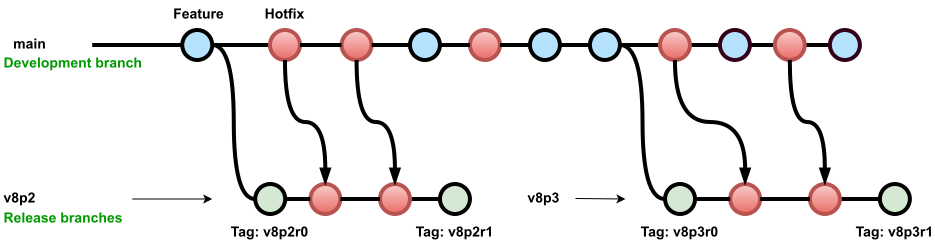
\includegraphics[scale=.6]{graphics/dev-cycle.png}
\caption{\label{fig_lifecycle}Development life cycle of the \telemacsystem{} version}
\end{figure}

\subsection{Version schedule}

\textbf{Version release}

The different versions, major and minor, are separated by a flexible interval:
\begin{itemize}
\item Major versions are released every 4 to 5 years.
\item Minor versions are released every year, if the amount of new developments
  is considered acceptable.
\end{itemize}

Finally, at any time we have the following versions:
\begin{itemize}
\item The development version: it is the \textbf{main} branch.
\item The latest stable version \textbf{vXpYrZ}.
\end{itemize}

This timetable can be modified due to a big change in the code that would
require longer validation to leave time for the normal integration to adapt.\\

\textbf{Removal of stable version}

The removal of a stable version is automatic when:
\begin{itemize}
  \item A corrective version \textbf{Z > 0} is released.
\item It reaches its expiration date.
\end{itemize}

\textbf{Maintained versions}

Only the last two minor versions are maintained.\\

\textbf{Exploitation version}

To do a study with the \telemacsystem{}, it is recommended to use the latest
stable version as it should be the most advanced and has the fewest bugs.

\subsection{Checklist for version release}

Here are the actions that need to be done when creating a new version
\textbf{vXpY}\@:
\begin{todolist}
\setlength\itemsep{0.01em}
  \item Create the branch \textbf{vXpY} from the main.
  \item Update the \verb!NEWS.txt!. Replace main section by section
    \textbf{vXpY}.
  \item In \verb!documentation/data/TelemacDoc.cls! change the command
    \verb!\telmaversion! to \textbf{vXpY}.
  \item In \verb!sources/utils/special/declarations_special.f! change the
    parameter VERSION to \textbf{vXpY}.
  \item In \verb!configs/systel.edf.cfg! change version to \textbf{vXpY}.
  \item Run \verb!compile_telemac.py --clean --rescan!. Update cmdf on main if necessary.
  \item Run \verb!validate_telemac.py!.
  \item Run \verb!validate_telemac.py --notebook --notebook-update!.
            Update content on the branch and also on main if necessary.
  \item Run \verb!doc_telemac.py!.
  \item Add all the generated documentation to repository.
  \item Run \verb!damocles.py --eficas!.
  \item Add the \verb!scripts/python3/eficas! folder to the repository.
\end{todolist}

Here are the actions that need to be done when creating a new version
\textbf{vXpYrZ}\@:
\begin{todolist}
\setlength\itemsep{0.01em}
  \item In the branch \textbf{vXpY} update \verb!NEWS.txt! with release date.
  \item Rerun Validation, documentation, eficas if some modifications where
    done to examples, documentation, dictionaries.
  \item Create the tag \textbf{vXpYrZ}.
\end{todolist}

